\RequirePackage{luatex85}
\documentclass[Ligatures=TeX,table,svgnames,usetotalslideindicator,compress,10pt,aspectratio=169]{beamer}
\usepackage{polyglossia}
\setdefaultlanguage{english}
\disablehyphenation
\usetheme{metropolis}
\usepackage{chemformula}
\setbeamertemplate{section in toc}[sections numbered]
\usepackage{slashbox}
\usepackage{fontawesome5}
\usepackage{tikz}
\usepackage{hyperref}
\usepackage[style=verbose,backend=biber]{biblatex}
\usepackage{multimedia}
\usepackage{algpseudocode}
\usepackage{algorithm}
\usepackage{amssymb}

\addbibresource{ref.bib}
\usepackage{appendixnumberbeamer}


\title{Scheduling dependent tasks within a smart city's fog/edge infrastructure powered by renewable energy}

\subtitle{ New Challenges in Scheduling Theory @ Aussois}

\author{\textbf{Miguel Vasconcelos}, Postdoc @ IRIT, Université de Toulouse, CNRS, Toulouse INP, UT3, Toulouse,France\\ 
 Georges Da Costa, IRIT, Université de Toulouse, CNRS, Toulouse INP, UT3, Toulouse, France\\
 Patricia Stolf, IRIT, Université de Toulouse, CNRS, Toulouse INP, UT3, Toulouse, France}
\institute
{
%  Postdoc at IRIT, Université de Toulouse, CNRS, Toulouse INP, UT3, Toulouse, France$^{1}$\\ 
}

\date{May 2024}
\renewcommand{\footnotesize}{\tiny}

\begin{document}
\setlength\abovecaptionskip{-3pt}

\frame{\titlepage}

\begin{frame}{Introduction}
\begin{columns}        
\begin{column}{0.5\textwidth}
  \begin{itemize}    
  \item Cloud-edge continuum
  \begin{itemize}
      \item Edge nodes with lower latency
      \item Possible to offload tasks to the cloud
  \end{itemize}
  \item Renewable energy
  \begin{itemize}
      \item Low power consumption of edge nodes
  \end{itemize}
  \item Smart-cities
  \begin{itemize}
      \item Applications often require low response time 
  \end{itemize}
  
  
 \end{itemize} 

\end{column}        
\begin{column}{0.5\textwidth}
      \begin{figure}[!h]
        \centering
        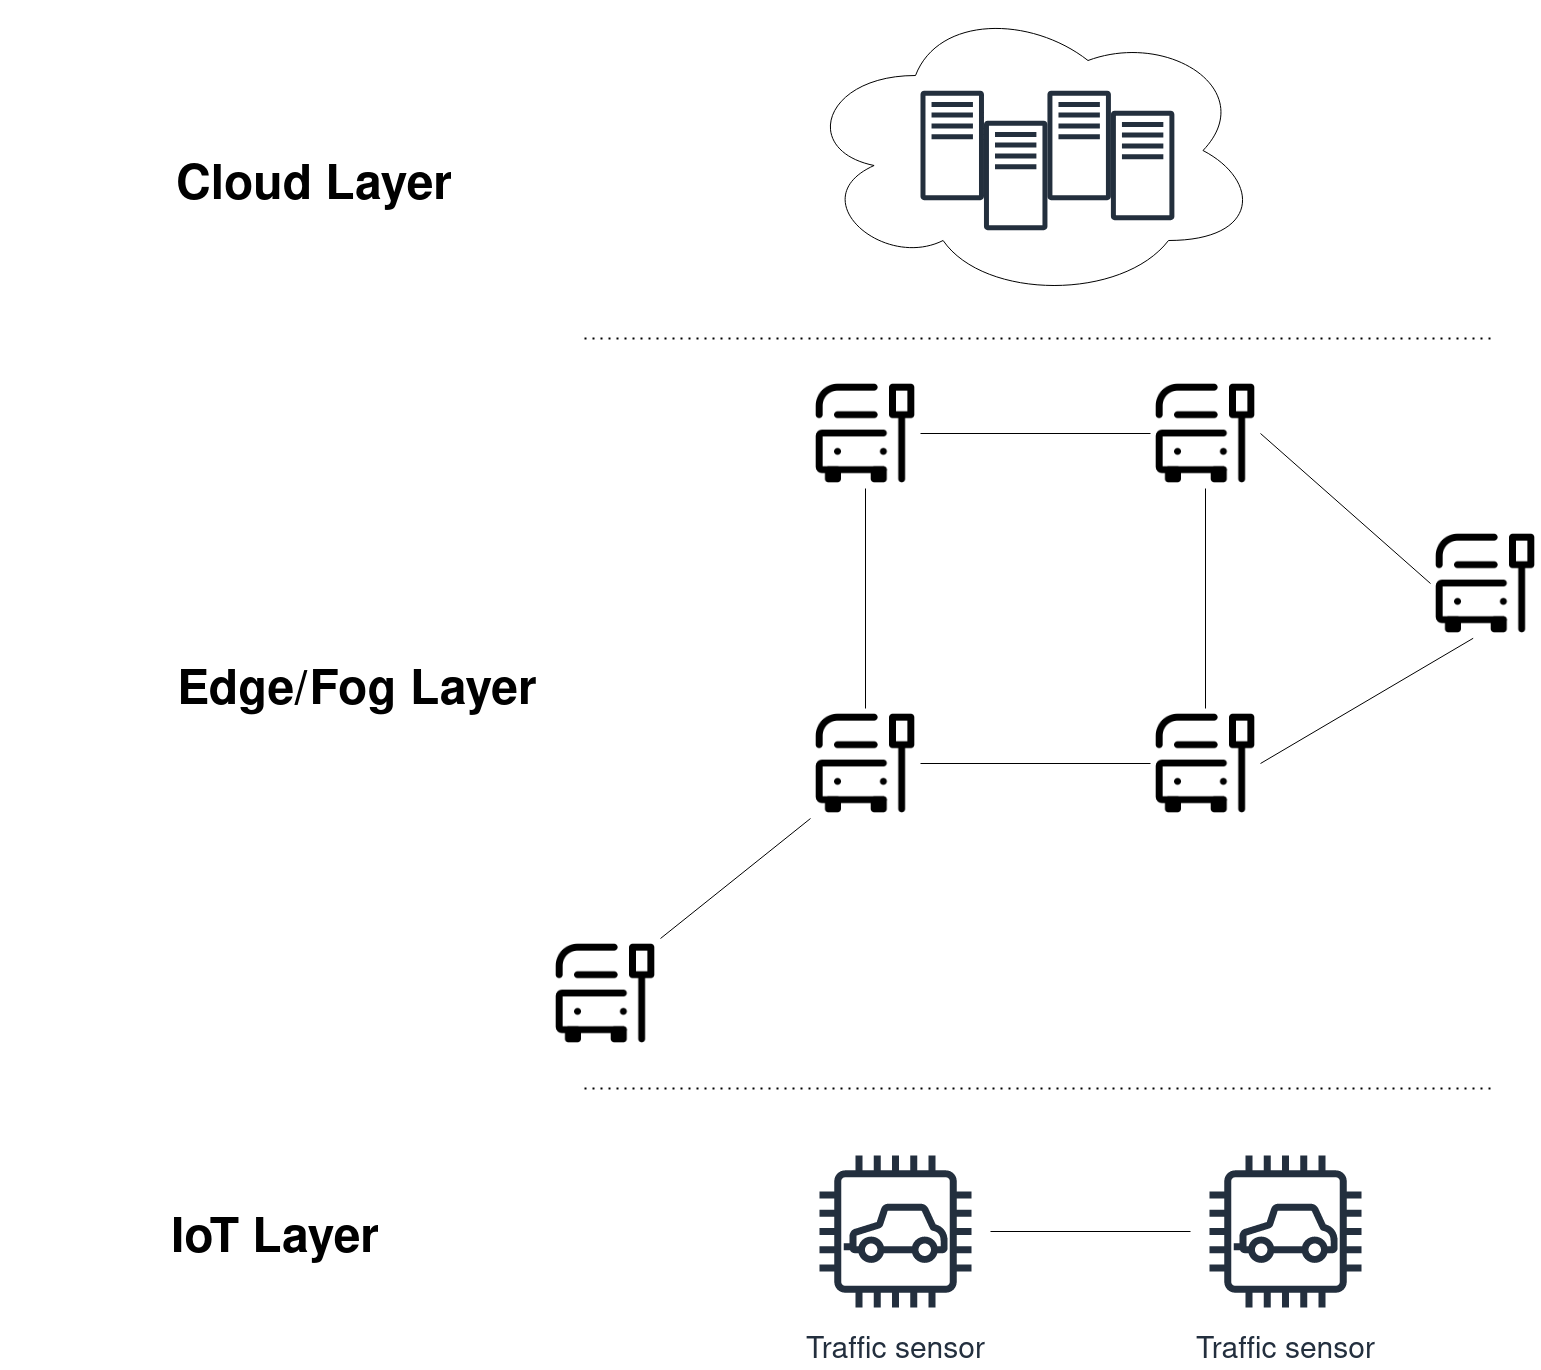
\includegraphics[width=\textwidth]{images/infrastructure.png}
        \caption{Cloud-Edge continuum in our context.}
      \end{figure}
    \end{column}        
\end{columns}


\end{frame}

\begin{frame}{Introduction}  

\begin{columns}
    
\begin{column}{0.6\textwidth}
\begin{itemize}
    \item \textbf{VILAGIL} project : improve mobility in Toulouse with smart city approach
    \item \textbf{Opportunistic computing}: Use the computational capacity already present in the city (computers at bus stops, metro stations ...)
    %\item Schedule tasks in the distributed edge/fog computing infrastructure
    \item Hosts supplied by renewable energy
  %  \item Optimize QoS, energy consumption, non-renewable energy consumption
\end{itemize}
    \end{column}


\begin{column}{0.5\textwidth}

   \begin{figure}[!h]
        \centering
        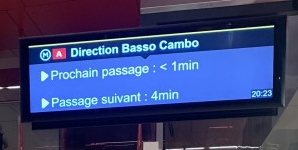
\includegraphics[width=.7\textwidth]{images/metro.png}
        \caption{Metro computer.}
      \end{figure}


   \begin{figure}[!h]
        \centering
        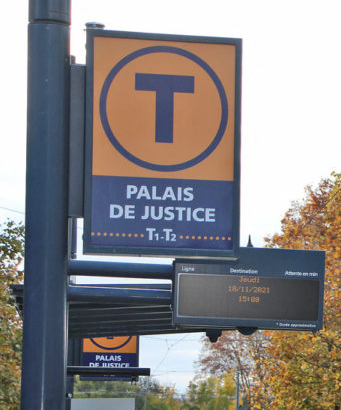
\includegraphics[width=.4\textwidth]{images/tramway.png}
        \caption{Tramway computer.}
      \end{figure}

\end{column}

\end{columns}


\end{frame}




\begin{frame}{Example of user request} 
\begin{columns}

\begin{column}{0.5\textwidth}

   \begin{figure}[!h]
        \centering
        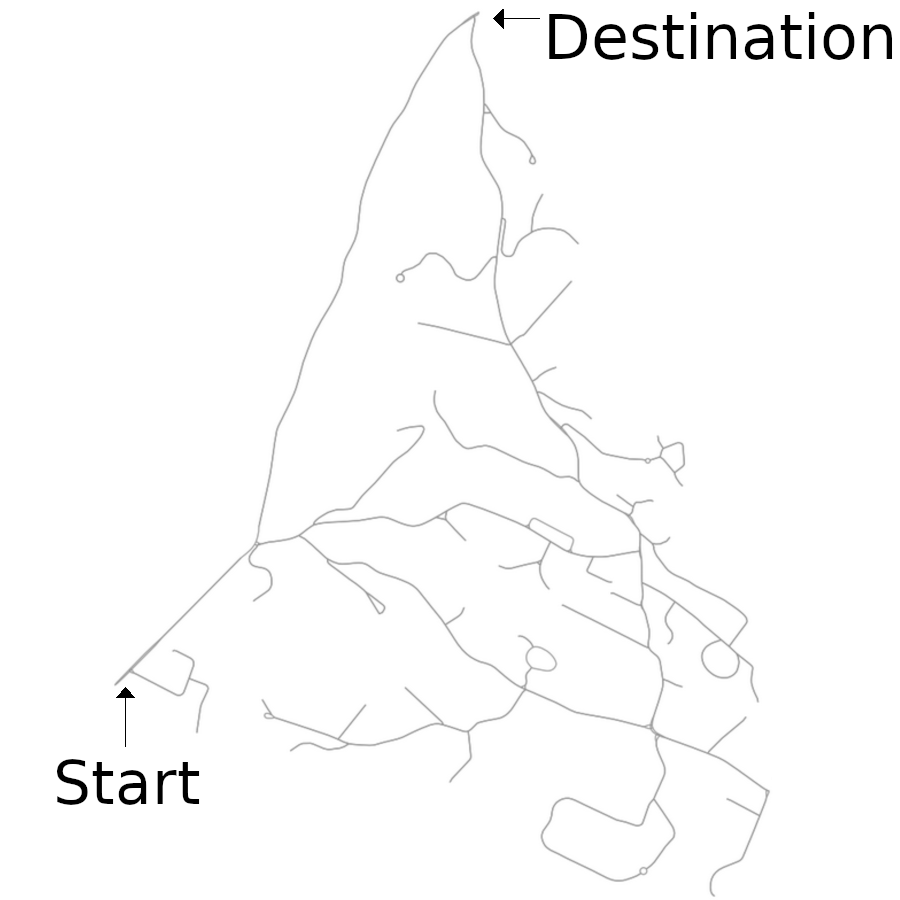
\includegraphics[width=\textwidth]{images/vieille_toulouse.png}
            \caption{Vieille-Toulouse map.}
      \end{figure}
      \end{column}
\begin{column}{0.5\textwidth}

\textbf{How long it takes from moving between the city ?}
\begin{itemize}
    \item Fuel consumed    
    \item \ch{CO2} emissions
    \item Costs
    \item Different modes of transportation
\end{itemize}
\pause
\textbf{Traffic prediction} : Essential information
\end{column}



\end{columns}
\end{frame}



\begin{frame}{Modeling a city} 
\begin{columns}

\begin{column}{0.5\textwidth}

   \begin{figure}[!h]
        \centering
        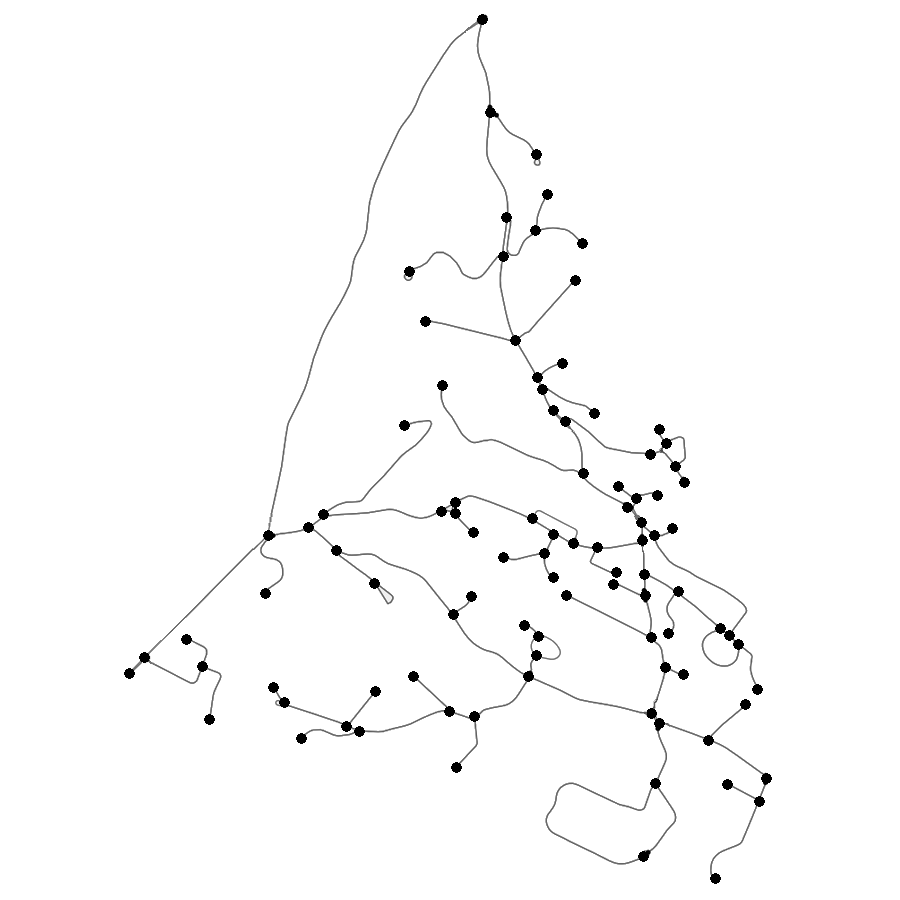
\includegraphics[width=\textwidth]{images/path_0.png}
        \caption{Street graph of Vieille-Toulouse.}
      \end{figure}
      \end{column}
\begin{column}{0.5\textwidth}
The city is represented as a \textbf{graph} of streets
\begin{itemize}
    \item  Edges are the streets
    \item Vertices are the interconnections between the streets
    
\end{itemize}

\end{column}

\end{columns}

\end{frame}




\begin{frame}{Example of a route} 
\begin{columns}        
  
\begin{column}{0.5\textwidth}

 \begin{figure}[]
        
        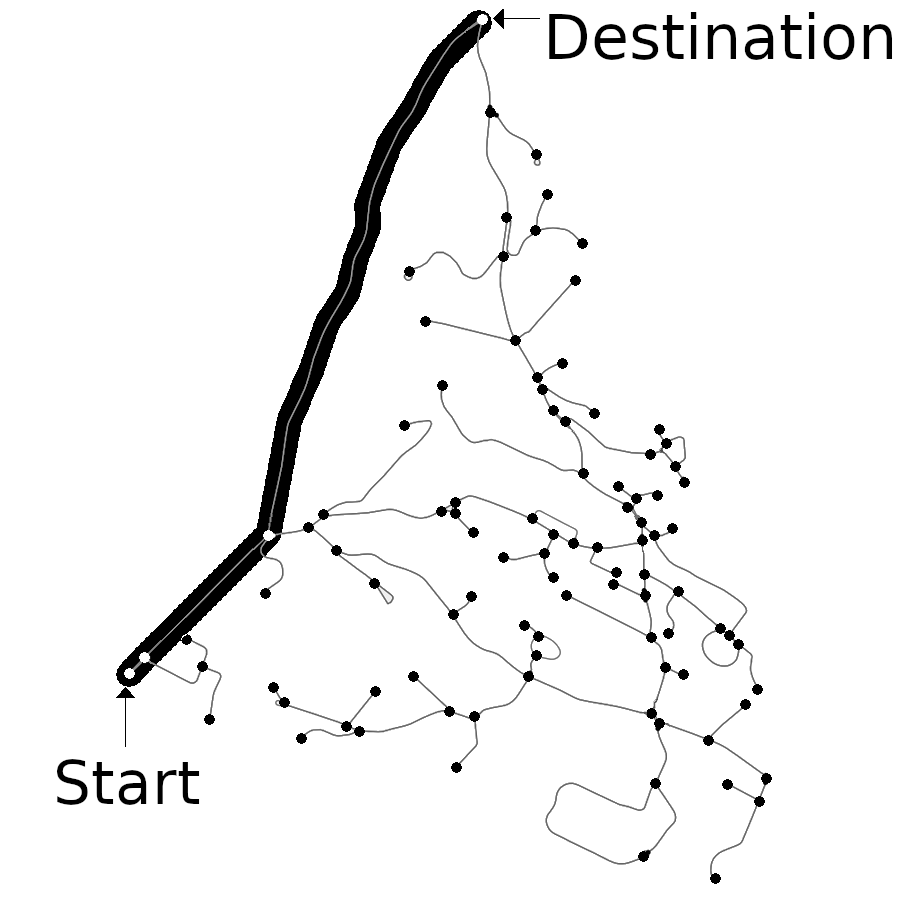
\includegraphics[width=\textwidth]{images/path_2.png}
        \caption{Example of a request.}
      \end{figure}
\end{column}
\begin{column}{0.5\textwidth}

   \begin{figure}[!h]
        \centering
        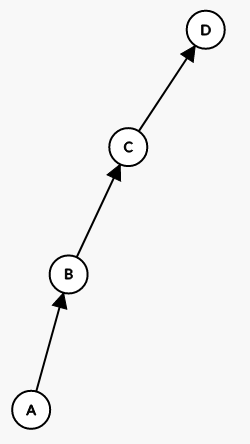
\includegraphics[width=.5\textwidth]{images/DAG_1.png}
        \caption{Tasks for the traffic computation.}
      \end{figure}
      
\end{column}

\end{columns}
\end{frame}



\begin{frame}{Example of a route - Impact of the other streets} 
\begin{columns}        
   
\begin{column}{0.5\textwidth}
\begin{figure}[!h]
        \centering
        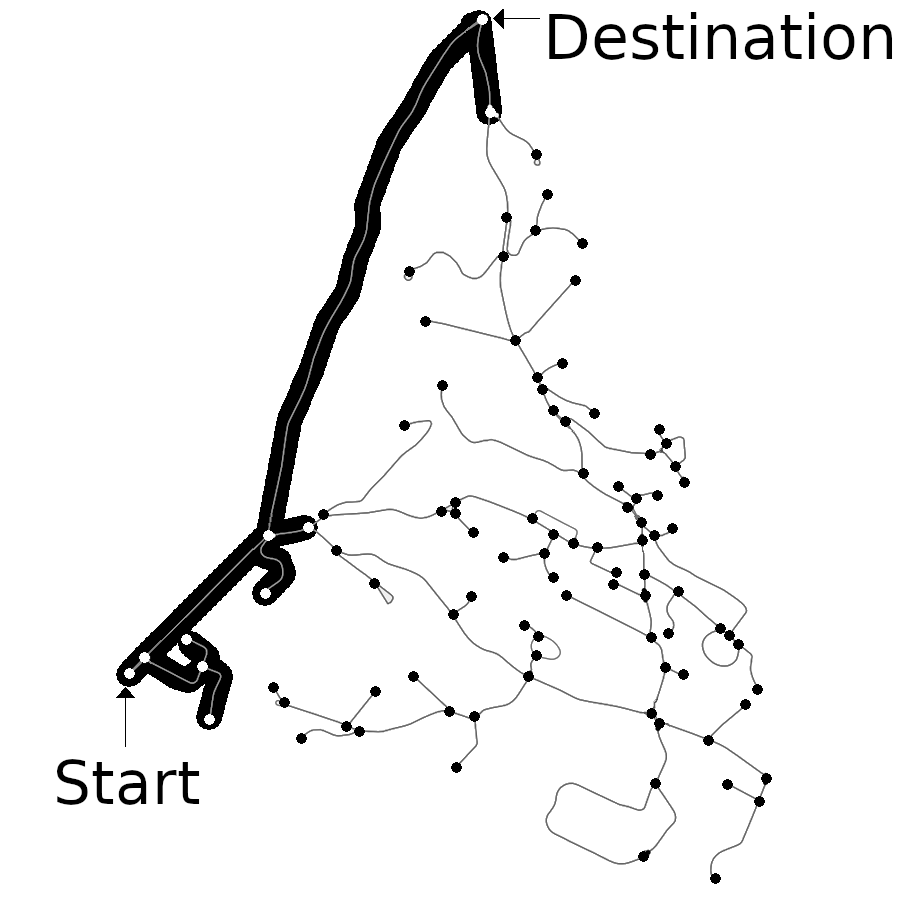
\includegraphics[width=\textwidth]{images/path_3.png}
        \caption{Example of one request.}
      \end{figure}

\end{column}
\begin{column}{0.5\textwidth}
   \begin{figure}[!h]
        \centering
        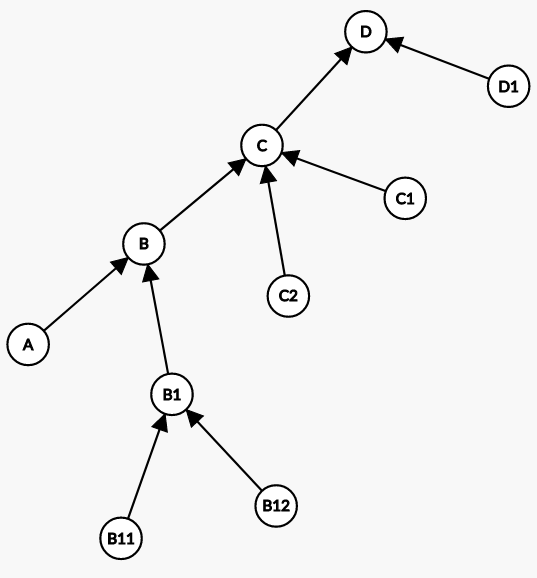
\includegraphics[width=.9\textwidth]{images/DAG_2.png}
        \caption{Tasks for the traffic computation.}
      \end{figure}
\end{column}

\end{columns}
\end{frame}

\addtocounter{framenumber}{-1}

\begin{frame}{Example of a route -  Source of the data} 
\begin{columns}        

\begin{column}{0.5\textwidth}
   \begin{figure}[!h]
        \centering
        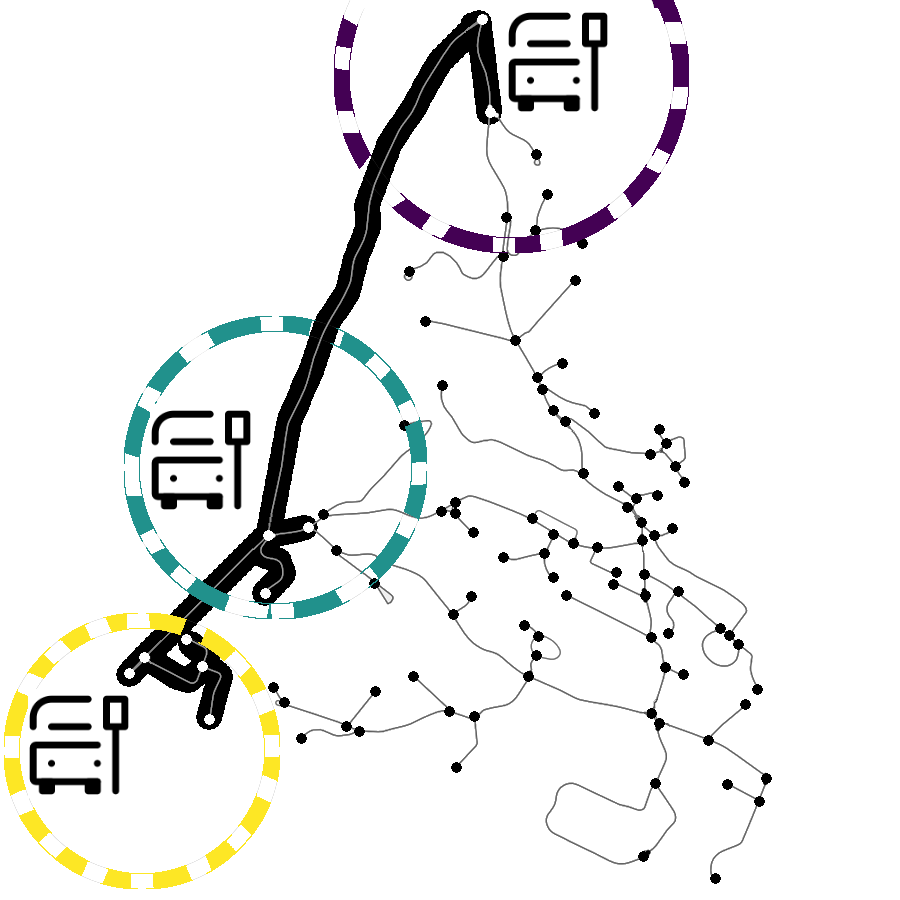
\includegraphics[width=\textwidth]{images/bus_stops_data.png}
        \caption{Example of one request.}
      \end{figure}

\end{column}
\begin{column}{0.5\textwidth}
   \begin{itemize}
       \item Traffic data is collected from the sensors around the city
       \item Each bus stop manages the data of the closest streets
       \item Communication is needed between the tasks to share the data
   \end{itemize}
\end{column}

\end{columns}
\end{frame}
\addtocounter{framenumber}{-1}
\begin{frame}{Example of a route -  Source of the data} 
\begin{columns}        

\begin{column}{0.5\textwidth}
   \begin{figure}[!h]
        \centering
        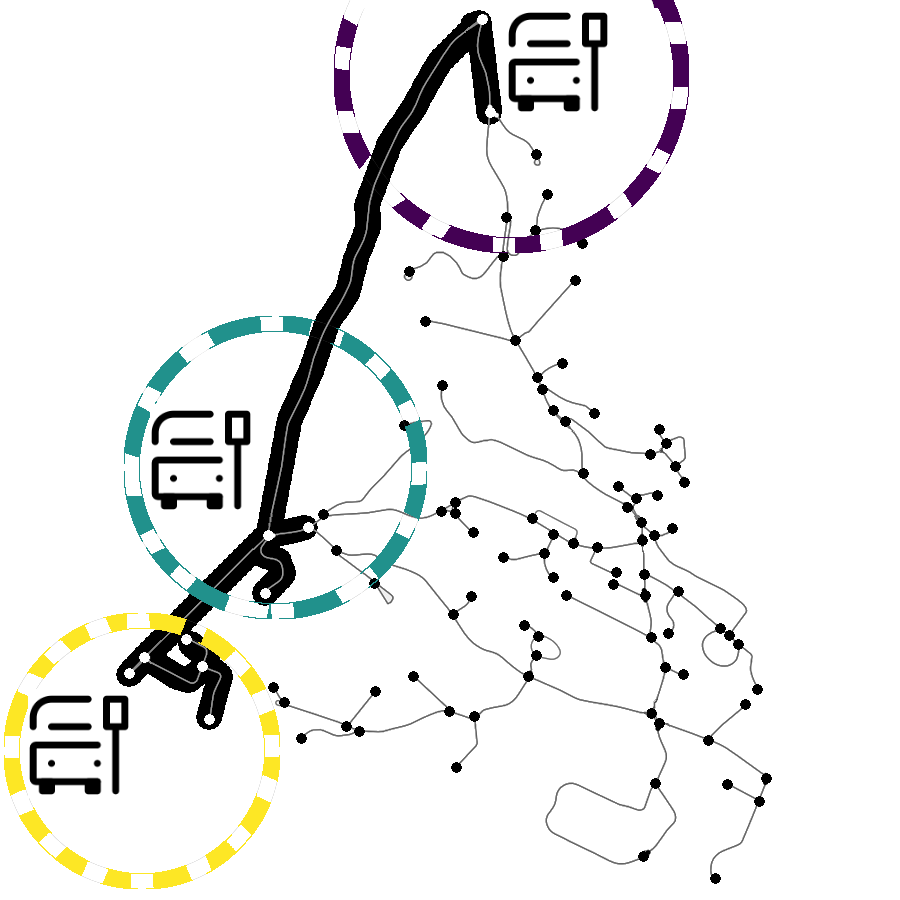
\includegraphics[width=\textwidth]{images/bus_stops_data.png}
        \caption{Example of one request.}
      \end{figure}

\end{column}
\begin{column}{0.5\textwidth}
   \begin{figure}[!h]
        \centering
        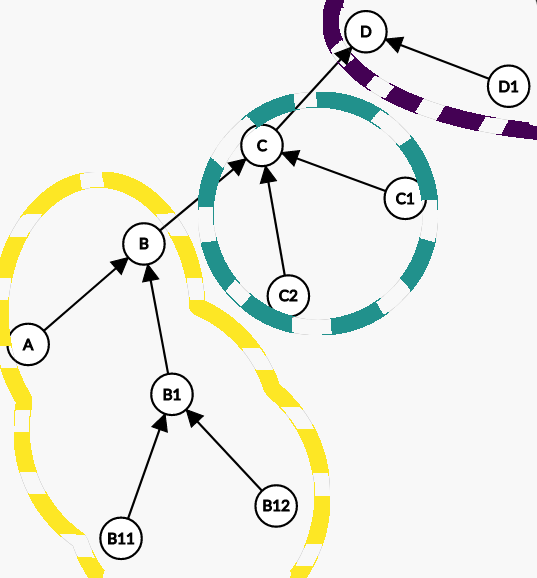
\includegraphics[width=.9\textwidth]{images/tasks_data.png}
        \caption{Tasks for the traffic computation.}
      \end{figure}
\end{column}

\end{columns}
\end{frame}

\begin{frame}{Requests and task model - Summary}
\begin{itemize}
    \item A user request about a path is represented as a Directed Acyclic Graph (DAG) of tasks
    \item Each task represents computation for a segment/street (prediction of traffic) 
    \item Each edge/fog node (bus stop) has local information of the streets (nearest streets)
    
\end{itemize}

\pause
\textbf{How to schedule the tasks to the fog/edge infrastructure aiming to reduce response time and non-renewable energy consumption ?}

\begin{itemize}
    \item Unrelated machines (different computing speeds, power consumption ...)
    \item Dependent tasks (prec), machine-dependent communication speeds (edge-edge, edge-cloud)
    
\end{itemize}


\end{frame}

\section{Experiments}

\begin{frame}{Initial Experiments}

\begin{itemize}
    \item Why the opportunistic approach? 
    \begin{itemize}
    \item Comparison between a centralized approach in terms of response time and energy consumption    
    \end{itemize}    
    \item How to schedule the workload in the distributed approach?
    \begin{itemize}
    \item Comparison between different algorithms in terms of response time, energy consumption and renewable energy usage   
    \end{itemize}    
\end{itemize}

\end{frame}

\begin{frame}{Experiment design and assumptions}

\begin{itemize}

    \item Computational simulations using the SimGrid framework\footnotemark[1]
    
    \item Tasks modeling:

    \begin{itemize}
        \item One tasks uses 100\% of one CPU core
        \item 0.1 s if executed in edge node; 0.05 s in the cloud
    \end{itemize}
    
    \item Network modeling:

    \begin{itemize}
        \item Flow-level TCP modeling
        \item No bandwidth limitations (TCP slow start not considered)
        \item Focus in network latency
    \end{itemize}

    \item Energy consumption:
    \begin{itemize}
        \item Linear model based on CPU usage
        \item Static part (idle) + dynamic part (based on CPU usage)
    \end{itemize}

\end{itemize}

\footnotetext[1]{Casanova, Henri, Giersch, Arnaud, Legrand, Arnaud, Quinson, Martin, Suter, Frédéric. Versatile, Scalable, and Accurate Simulation of Distributed Applications and Platforms. Journal of Parallel and Distributed Computing, 2014.}
  \end{frame}

  \section{Experiment I : Centralized vs distributed}
\begin{frame}{Computational infrastructure modeling}


%Network links latency:
 % \begin{itemize}
  %    \item 0.01 seconds between the nodes
  %\end{itemize}
%\vspace{1cm}
\begin{columns}        
\begin{column}{0.5\textwidth}

%Computational simulations %developed using the SimGrid framework
%\begin{itemize}
 % \item Validated models for network and energy
%end{itemize}


\textbf{Centralized approach:}
  \begin{itemize}    
  \item  Server with 64 CPU cores
  \item 66 W when idle; 220 W at 100\% %of utilization
  \end{itemize}    
  \textbf{Distributed approach:} 
  \begin{itemize}    
  \item 17 Raspberry PI with 4 CPU cores each
  \item 2.5 W when idle; 7.3 W at 100\% 
  \item (total of 42.5 W when idle, and 124.1 W at 100\%)
  \item Network links latency:
  \begin{itemize}
      \item 10 ms between edge nodes
  \end{itemize}
  \end{itemize}

 
  \end{column}
  \begin{column}{0.5\textwidth}

  
   \begin{figure}[!h]
        \centering
        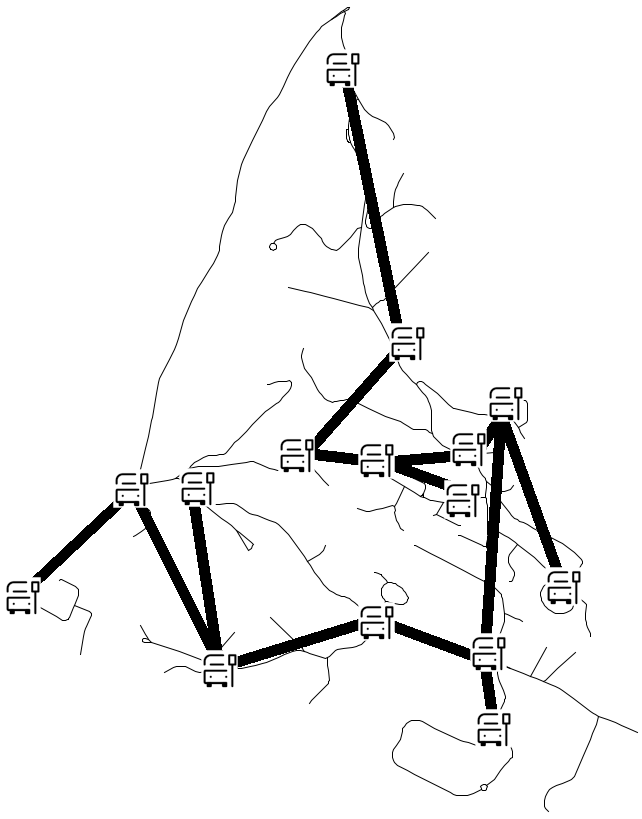
\includegraphics[width=.8\textwidth]{images/vieille-toulouse.png}
        \caption{Distributed  infrastructure.}
      \end{figure}

  
    \end{column}
\end{columns}
  \end{frame}



\begin{frame}{Workload}
\begin{columns}        
\begin{column}{0.4\textwidth}

  \begin{itemize}
      \item Inspired by real mobility data \footnotemark[2]
      \item 30000 requests 
  \end{itemize}
  \end{column}
\begin{column}{0.6\textwidth}

    \begin{figure}[!h]
    \centering
    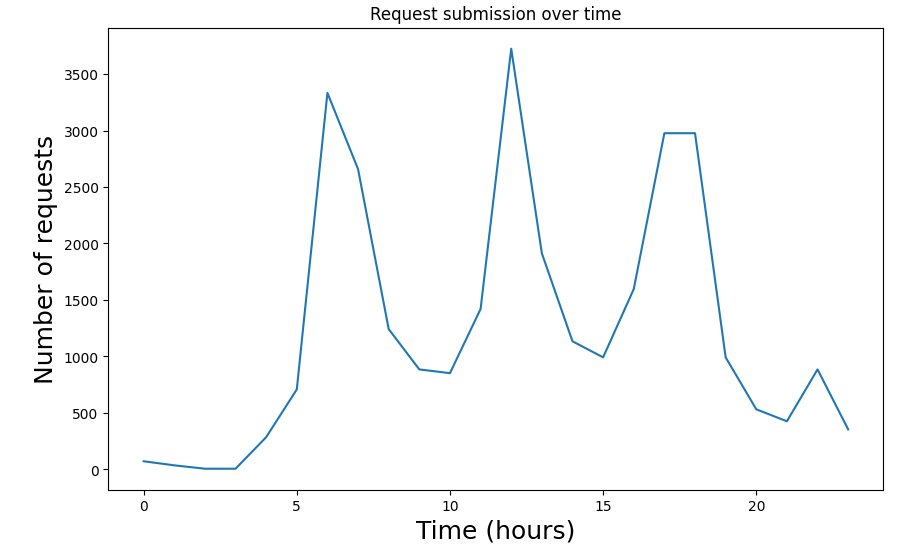
\includegraphics[width=\textwidth]{images/workload.png}
    \caption{Workload distribution}
    
  \end{figure}
    \end{column}
  \end{columns}

\footnotetext[2]{Metro SP, Pesquisa Origem e Destino 2017.}
  \end{frame}



\begin{frame}{Results}
  \begin{columns}

  \begin{column}{0.5\textwidth}

Using the distributed version:
\begin{itemize}
    \item \textbf{35\% of energy savings} 
    \item Average \textbf{response time reduced by 40\%}
    \begin{itemize}
    \item Tasks executed closer to where the data is produced
    \end{itemize}
\end{itemize}

  \end{column}
  \begin{column}{0.5\textwidth}

  
   \begin{figure}[!h]
        \centering
        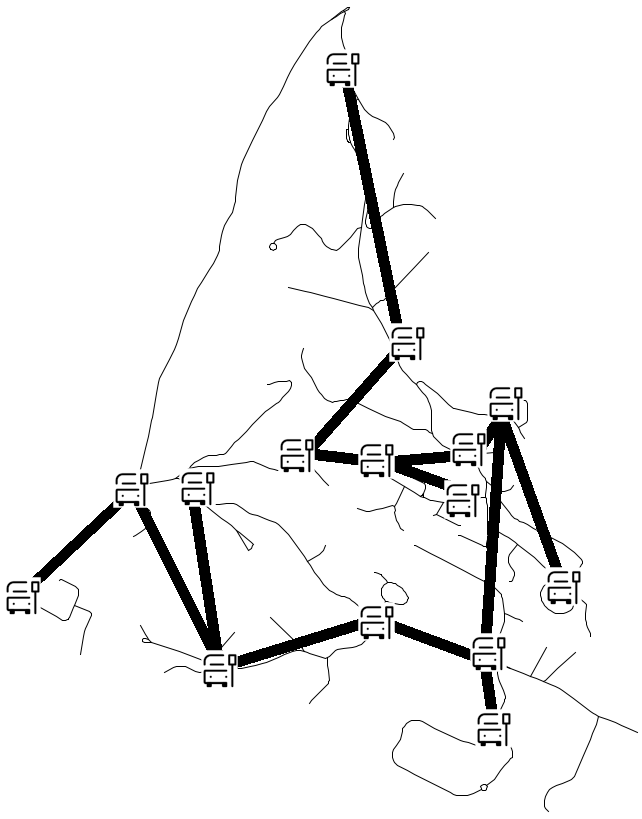
\includegraphics[width=.8\textwidth]{images/vieille-toulouse.png}
        \caption{Distributed  infrastructure.}
      \end{figure}

  
    \end{column}
\end{columns}

\end{frame}



\section{Experiment II :Different scheduling algorithms for the distributed approach}
  
\begin{frame}{Computational infrastructure modeling}
\begin{columns}        
\begin{column}{0.5\textwidth}

  \begin{itemize}    
  \item 17  Raspberry PI with 4 CPU cores (fog/edge):  2.5 W when idle; 7.3 W at 100\% 
  \item Server with 256 CPU cores (cloud): 66 W when idle; 220 W at 100\%
  \item Network links latency:
  \begin{itemize}
      \item 10 ms for edge/fog
      \item 100 ms for cloud
  \end{itemize}

  \end{itemize}    
  \end{column}
  \begin{column}{0.5\textwidth}

    \begin{figure}[!h]
    \centering
    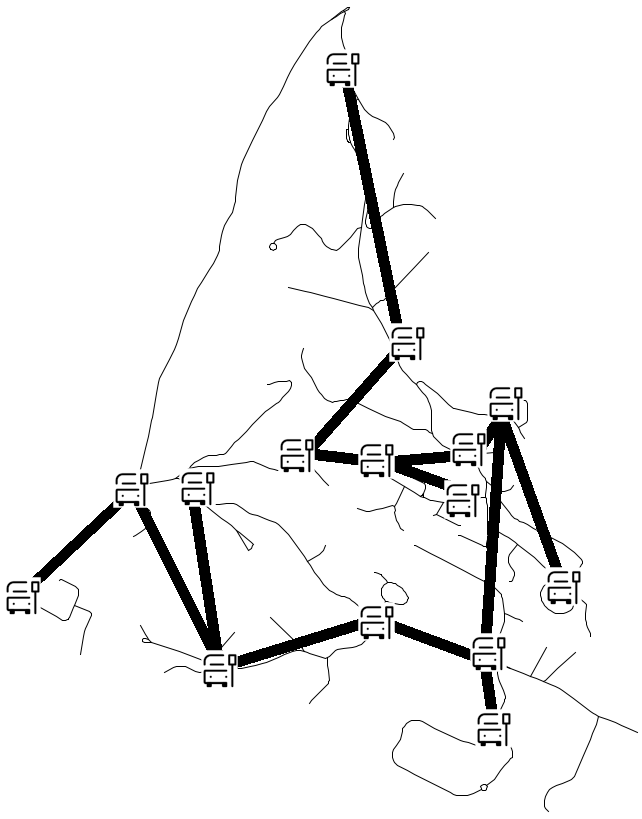
\includegraphics[width=.8\textwidth]{images/vieille-toulouse.png}
    \caption{Edge/Fog infrastructure}
  \end{figure}
    \end{column}
\end{columns}
  \end{frame}

\begin{frame}{Algorithms}
 \textbf{Baseline}
  \begin{itemize}
      \item Allocate to the bus stop that have its required data
      \item (less communications)
  \end{itemize}

\textbf{   Heterogeneous Earliest Finish Time (HEFT)}\footnotemark[3]  \begin{itemize}
      \item Allocate to the host with that will have the earliest finish time (considering computations and communications)    
  \end{itemize}


\textbf{   Green Earliest Finish Time (GEFT)}  \begin{itemize}
      \item Allocate to the host that have green energy and the earliest finish time 
      \item inspired in the HEFT algorithm
  \end{itemize}

\footnotetext[3]{Topcuoglu, Haluk; Hariri, Salim; Wu, M. (2002). `Performance-effective and low-complexity task scheduling for heterogeneous computing''. IEEE Transations on Parallel and Distributed Systems. 13 (3): 260–274}
  \end{frame}



\begin{frame}{Energy modeling}
\begin{itemize}
  \item Edge hosts have PV panels and batteries, and use grid as backup
  \item Electricity from the grid is assumed to be carbon intensive, and renewable from the cloud layer    
    \item Solar irradiation values per minute (NASA MERRA-2)\footnotemark[3]
    \item Small variation of irradiation between the different hosts (considering a city)
\end{itemize}
      \begin{figure}[!h]
        \centering
        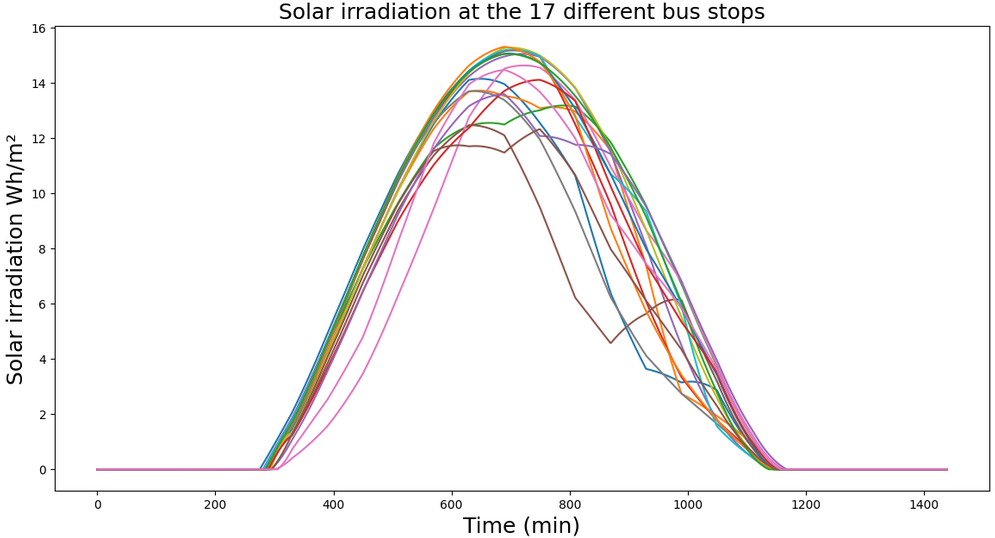
\includegraphics[width=.6\textwidth]{images/solar_energy.png}
        \caption{Solar irradiation values}
      \end{figure}

  \footnotetext[3]{Global Modeling and Assimilation Office (GMAO) (2015), MERRA-2 tavg1\_2d\_slv\_Nx: 2d,1-Hourly,Time-Averaged,Single-Level,Assimilation,Single-Level Diagnostics V5.12.4, Greenbelt, MD, USA, Goddard Earth Sciences Data and Information Services Center (GES DISC), Accessed: 26\/03\/2024 DOI:10.5067\/VJAFPLI1CSIV}
  \end{frame}


\begin{frame}{Results - Requests response time}

\begin{table}[h]
  
  \caption{Statistics of the request response time (is seconds) by algorithm }\label{tab:dcutilization} \centering

  \begin{tabular}{|l|r|r|r|r|r|}
   \hline
    
   \textbf{Alg.} &   \textbf{Mean} & \textbf{Median} & \textbf{90\%} & \textbf{95\%}& \textbf{99\%} \\
  \hline
  Baseline  & 7.75 & 1.02  & 28.15 & 38.25 & 56.52 \\
  \hline
  HEFT  & 0.74 &  0.73 & 0.98 & 0.99 &  1.07 \\
  \hline
  GEFT & 0.82 & 0.84  & 1.02 & 1.04 & 1.28 \\
  \hline
  
\end{tabular}  
\end{table}
\end{frame}



\begin{frame}{Results - Task allocation}

   \begin{figure}[!h]
        \centering
        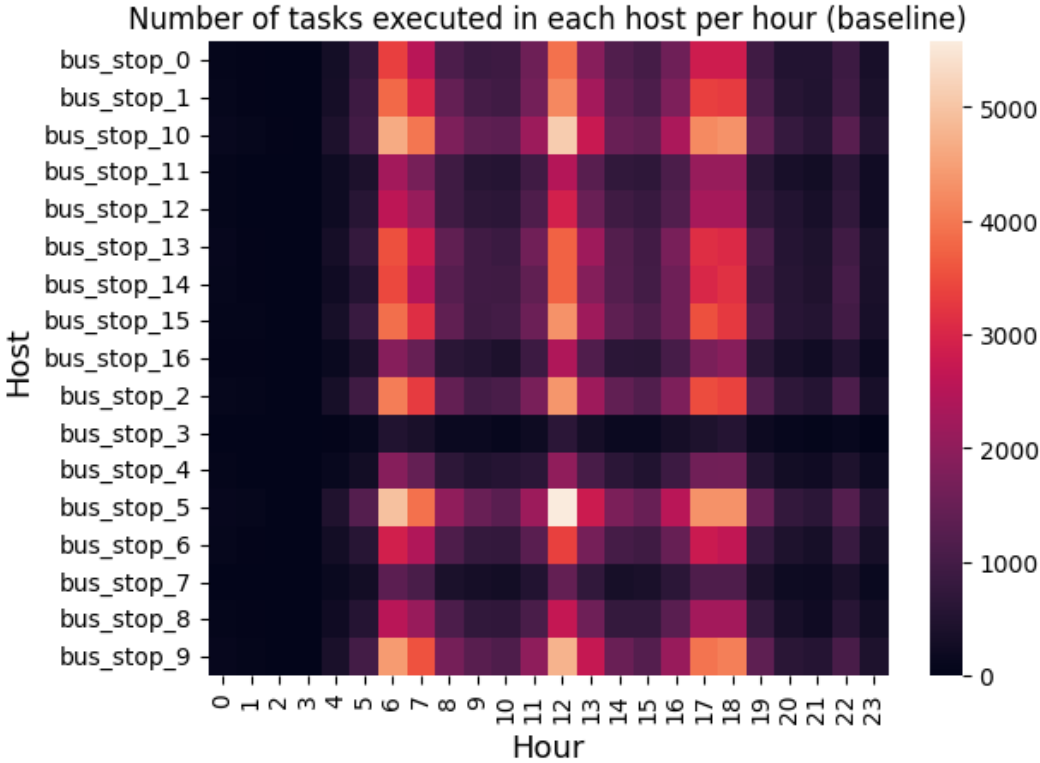
\includegraphics[width=.7\linewidth]{images/baseline.png}
        \caption{Task allocation over time for the baseline algorithm.}
      \end{figure}

\end{frame}

\begin{frame}{Results - Task allocation}

   \begin{figure}[!h]
        \centering
        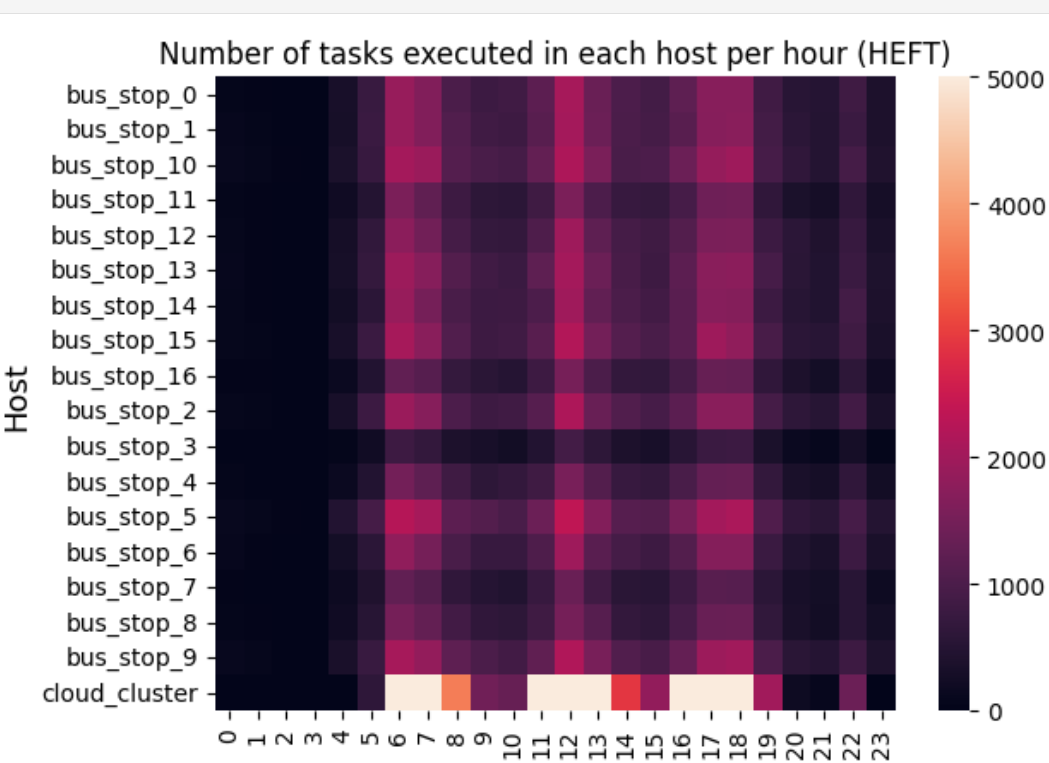
\includegraphics[width=.7\linewidth]{images/heft.png}
        \caption{Task allocation over time for the HEFT algorithm.}
      \end{figure}

\end{frame}

\begin{frame}{Results - Task allocation}

   \begin{figure}[!h]
        \centering
        \includegraphics[width=.7\linewidth]{images/GEFT.png}
        \caption{Task allocation over time for the GEFT algorithm.}
      \end{figure}

\end{frame}


\begin{frame}{Results - Energy consumption}

\begin{table}[h]
  
  \caption{Energy consumption by algorithm }\label{tab:dcutilization} \centering

  \begin{tabular}{|l|r|r|r|r|r|}
   \hline
    
   \textbf{Alg.} &   \textbf{Total (Wh)} & \textbf{Non-Renewable (Wh)} & \textbf{Renewable energy usage (\%)}\\
  \hline
  Baseline  & 29.87 & 5.98 &  80\% \\
  \hline
  HEFT  & 30.69 &  3.99 & 87\% \\
  \hline
  GEFT & 36.08 & 0.08  &    99.7\% \\
  \hline

\end{tabular}
\end{table}

*Results without Idle time

\end{frame}

\begin{frame}{Summary}

\begin{itemize}
    \item Scheduling dependent tasks into a fog/edge infrastructure
    \item Presence of renewable energy in the hosts
    \item Improve QoS
    \item Increase renewable energy usage
\end{itemize}
\end{frame}



\begin{frame}{Ongoing work}



\begin{columns}

\begin{column}{0.5\textwidth}

   \begin{figure}[!h]
        \centering
        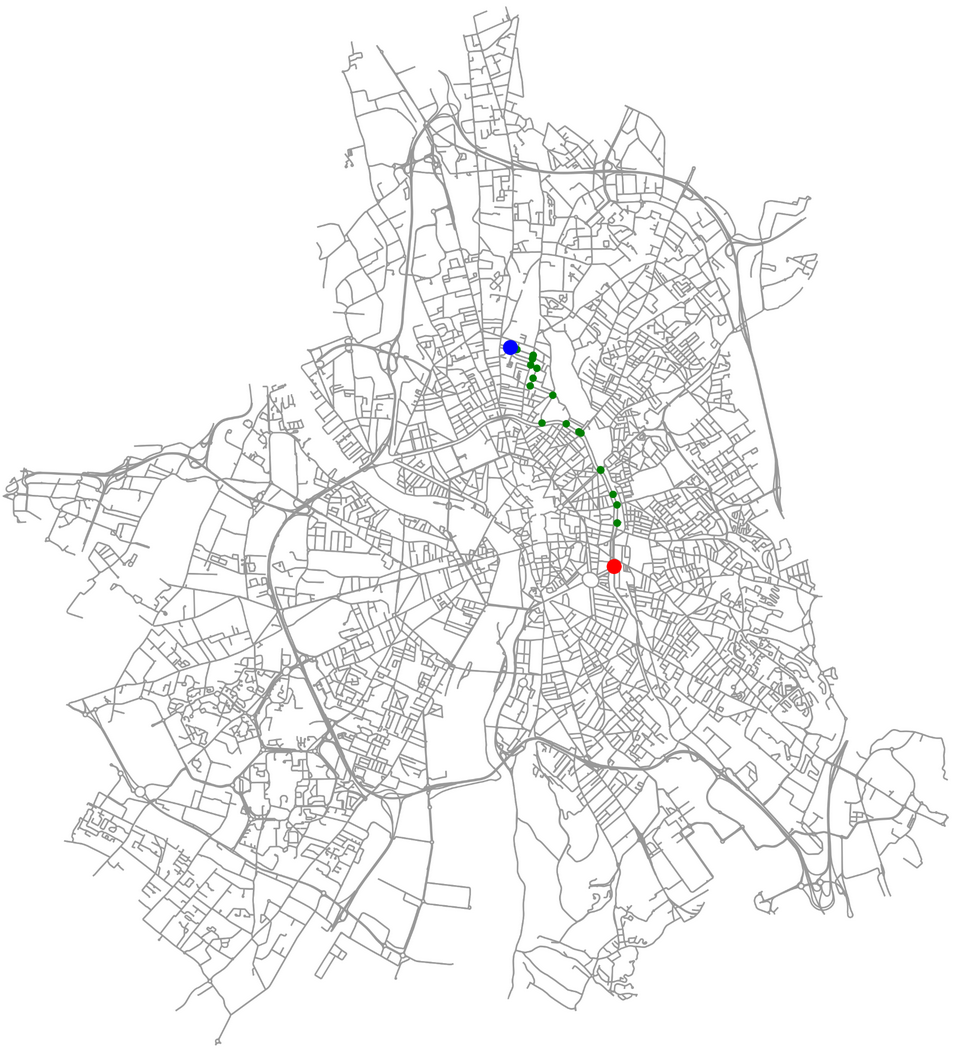
\includegraphics[width=.94\textwidth]{images/toulouse_path.png}
        \caption{Example of path in Toulouse.}
      \end{figure}
      \end{column}
\begin{column}{0.5\textwidth}
Considering Toulouse
\begin{itemize}
    \item 1638 hosts (open street map)
    \begin{itemize}
        \item bus stops
        \item tram stops
        \item metro stations
        \item train stations
    \end{itemize}
\end{itemize}
\end{column}
\end{columns}

\end{frame}



\begin{frame}{Ongoing work}

\begin{columns}

\begin{column}{0.5\textwidth}

   \begin{figure}[!h]
        \centering
        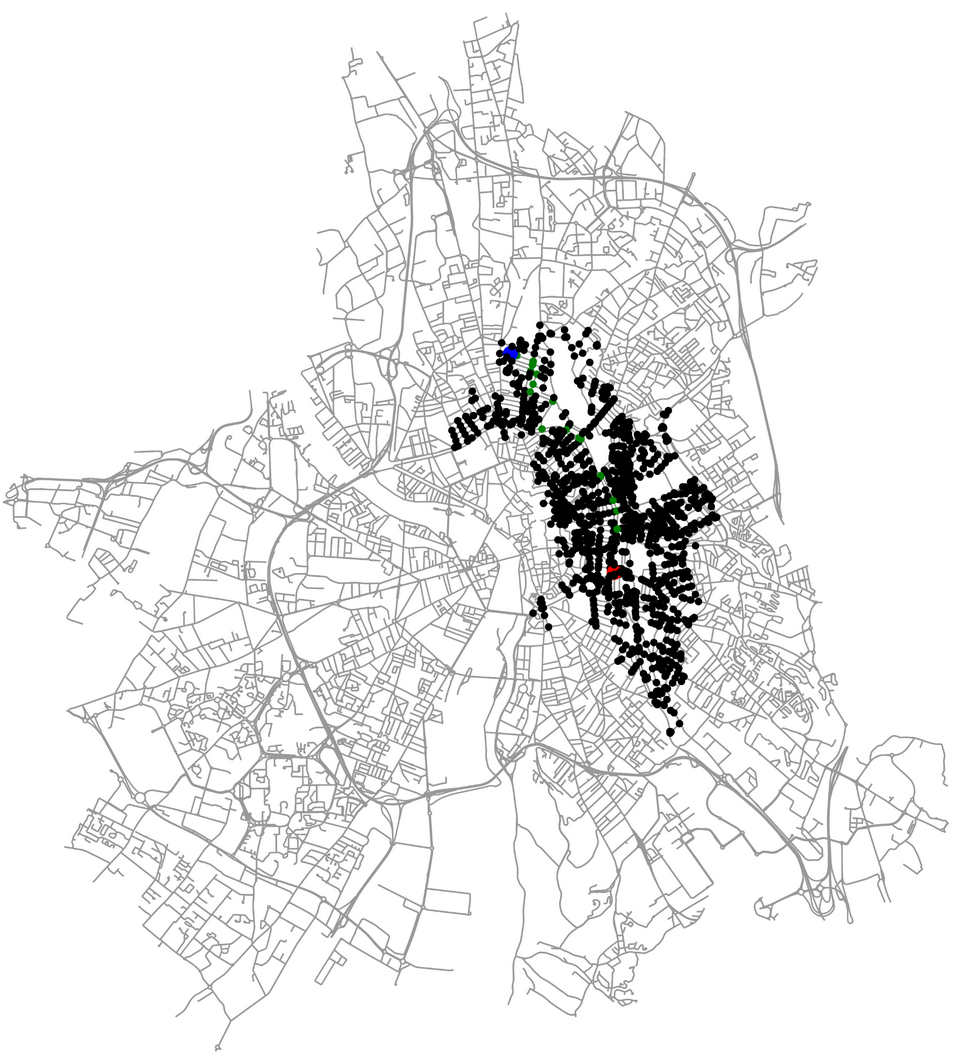
\includegraphics[width=.94\textwidth]{images/toulouse_path_alltasks.png}
        \caption{Example of path in Toulouse.}
      \end{figure}
      \end{column}
\begin{column}{0.5\textwidth}
Considering Toulouse
\begin{itemize}
    \item 1638 hosts (open street map)
    \begin{itemize}
        \item bus stops
        \item tram stops
        \item metro stations
        \item train stations
    \end{itemize}
    \item Requests with more tasks to execute: 6949 tasks in the example


\end{itemize}

\end{column}

\end{columns}

\end{frame}

\begin{frame}{Benefits and challenges of simulations}

\begin{itemize}
    \item Execution time of simulations (using a laptop) 
    \begin{itemize}
        \item  2 minutes (centralized, baseline), 8 minutes (GEFT, HEFT) to simulate one day
        \item 1 CPU core (possibility to run longer periods of time in parallel)
    \end{itemize}
    \item Challenges in network modeling :
    \begin{itemize}
        \item  Mobile network modeling, mobility of nodes in space, dynamic latency
    \end{itemize}
    
\end{itemize}

\end{frame}

\begin{frame}{Other future Research directions}

\begin{itemize}
    \item Shutdown idle hosts and manage the workload to the other hosts
    \item Caching
    \item Other scheduling strategies
    \item Information of the climate conditions and users requests in the scheduling decision
   % \item Offload tasks to the cloud
    \item Adding new servers in the edge layer and the trade-off between costs (\$, \ch{CO2}) and QoS
\end{itemize}
\end{frame}

\appendix

\begin{frame}{Acknowledgments}
  \begin{itemize}
  \small
   \item  GIS neOCampus of Université Toulouse III Paul Sabatier
   \item This work was carried out within the MaaS action of the VILAGIL project, a project co-financed by Toulouse Métropole and France 2030 as part of the Territoires d'innovation program operated by the Banque des territoires
  \end{itemize}    
    \begin{center}
    \begin{figure}[h]    
      \centering
      
\includegraphics[width=\textwidth]{images/ack4.png}
      \caption{Funding projects and agencies}
    \end{figure}    
  \end{center}  

\end{frame}



\begin{frame}{Thank you !}


\textbf{Thank you for your attention!}\\
Contact: miguel-felipe.silva-vasconcelos@irit.fr

\par\noindent\rule{\textwidth}{0.5pt}

\begin{center}

\textbf{Scheduling dependent tasks within a smart city's fog/edge infrastructure powered by renewable energy}

Miguel Felipe Silva Vasconcelos

Postdoc @ IRIT, Université de Toulouse, CNRS, Toulouse INP, UT3, Toulouse, France \\
\end{center}

\end{frame}

\appendix
\begin{frame}{Results - Requests response time}

\begin{table}[h]
  
  \caption{Statistics of the request response time (is seconds) by algorithm }\label{tab:dcutilization} \centering

  \begin{tabular}{|l|r|r|r|r|r|}
   \hline
    
   \textbf{Alg.} &   \textbf{Mean} & \textbf{Median} & \textbf{90\%} & \textbf{95\%}& \textbf{99\%} \\
  \hline
  Baseline  & 7.75 & 1.02  & 28.15 & 38.25 & 56.52 \\
  \hline
  Baseline (Vivaldi)  & 4.20  & 0.785  & 14.61 & 21.48 &  32.22 \\
  \hline
  Centralized  & 10.49 & 1.18  & 35.16 & 43.41 & 60.10 \\
  \hline
  Centralized (Vivaldi)  & 1.45  & 0.53  & 3.055 & 7.29 &  13.23 \\
  \hline
  
\end{tabular}  
\end{table}
    \end{frame}

\begin{frame}{Results - Requests response time}

\begin{table}[h]
  
  \caption{Statistics of the request response time (is seconds) by algorithm }\label{tab:dcutilization} \centering

  \begin{tabular}{|l|r|r|r|r|r|}
   \hline
    
   \textbf{Scenario} &   \textbf{Mean} & \textbf{Median} & \textbf{90\%} & \textbf{95\%}& \textbf{99\%} \\
  \hline
  Opportunistic & 4.20  & 0.785  & 14.61 & 21.48 &  32.22 \\
  \hline
  Centralized  & 1.45  & 0.53  & 3.055 & 7.29 &  13.23 \\
  \hline
  
\end{tabular}  
\end{table}
    \end{frame}



\end{document}

